% vim: ai sw=2 textwidth=78 spell spelllang=en

\documentclass[handout,xcolor=dvipsnames]{beamer}

\let\Oldemph\emph
\renewcommand{\emph}[1]{\textcolor{blue}{\Oldemph{#1}}}
\newcommand{\heading}[1]{\textbf{\textcolor{BurntOrange}{#1}}}

% Copyright 2004 by Till Tantau <tantau@users.sourceforge.net>.
%
% In principle, this file can be redistributed and/or modified under
% the terms of the GNU Public License, version 2.
%
% However, this file is supposed to be a template to be modified
% for your own needs. For this reason, if you use this file as a
% template and not specifically distribute it as part of a another
% package/program, I grant the extra permission to freely copy and
% modify this file as you see fit and even to delete this copyright
% notice.


\mode<presentation>
{
%  \usetheme{Warsaw}
\usetheme{Madrid}

  \setbeamercovered{transparent}
}

\usepackage[utf8]{inputenc}
\usepackage{times}
\usepackage[IL2]{fontenc}

\usepackage{graphicx}
\usepackage[final]{listings}
\usepackage{multirow}

\lstset{tabsize=2,numbers=none,showstringspaces=false,breaklines=true,
	breakatwhitespace=true,escapeinside={(*@}{@*)},
	basicstyle=\scriptsize,keywordstyle=\bfseries\color{OliveGreen},
	commentstyle=\color{blue}}

\title{Kernel Testing -- Static Analysis}

\subtitle{\ldots and not only the kernel}

\author[J. Slaby]{\emph{Jiri~Slaby}}

\institute{Suse Labs, Novell}

\date[7/14/2010, Prague]{Prague, July 14 2010}

\begin{document}

\begin{frame}
  \titlepage
\end{frame}

%%%%%%%%%%%%%%%%%%%%%%%

\begin{frame}
  \frametitle{Outline}
  \begin{itemize}
  \item Introduction, motivation
  \item State of the art
  \item Kernel checking methods
  \begin{itemize}
  \item Checking SUSE kernels?
  \end{itemize}
  \end{itemize}
\end{frame}

\begin{frame}
  \frametitle{Introduction, motivation I.}
  \heading{Who the presenter is?}
  \begin{itemize}
  \item Labs member
  \item PhD student, researching:
  \begin{itemize}
  \item static analysis
  \item its application to the kernel
  \end{itemize}
  \end{itemize}

  \medskip
  \pause

  \heading{Static analysis}
  \begin{itemize}
  \item Without \emph{really} executing the code
  \item Opposite to dynamic analysis/testing
  \item Performed by tools
  \item What is it good for?
  \begin{itemize}
  \item No dependency on input = all branches analyzed (higher coverage)
  \item No requirements (like HW for drivers testing etc.)
  \end{itemize}
  \end{itemize}

\end{frame}

\begin{frame}[fragile]
  \frametitle{Introduction, motivation II.}
  \heading{Uses}
  \begin{itemize}
  \item Optimization $\Rightarrow$ compilers
  \item Bug-finding $\Rightarrow$ checkers (and compilers)
  \end{itemize}

  \pause
  \medskip

  \heading{Example}
  \begin{center}
  \begin{tabular}{c}
  \begin{lstlisting}[language=C]
int a = 0, b = read_int();
return a / b;
  \end{lstlisting} \\
  $\Downarrow$
  \end{tabular} \\
  \pause
  \begin{tabular}{|l|l|} \hline
  \emph{Compiler} & \onslide<4->{\emph{Checker}} \\ \hline
  \begin{lstlisting}[language=C]
return 0;
  \end{lstlisting} & \pause
  \begin{lstlisting}[language=C]
int a = 0, b = read_int();
__PROVE__(b != 0);
return a / b;
  \end{lstlisting} \\ \hline
  Better code & \onslide<4->{Press "0" to crash it!} \\ \hline
  \end{tabular}
  \end{center}

  \pause

  \begin{center}
  Generally undecidable (can be reduced to the halting problem)

  \pause
  \medskip

  \heading{Generally!}
  \end{center}

\end{frame}

\part{State of the Art}

\begin{frame}
  \partpage
\end{frame}

\begin{frame}[fragile]
  \frametitle{State of the Art I.}
  \heading{What analyses are currently used?}
  \begin{itemize}
  \item[(1)] Flow analyses
  \begin{itemize}
  \item Walk built structures (AST, CFG, call-graph)
  \item Use automata or similar to find bugs
  \item Some count fix-points of a system of equations
  \item Prone to false-positives
  \item Examples: \textsc{Coverity}, \textsc{Sparse}, \textsc{Stanse},
  \textsc{Clang}
  \end{itemize}
  \end{itemize}

  \begin{center}
  \begin{tabular}{ccccccc}
  \begin{lstlisting}[language=C]
lock();
if (X)
  return;
unlock();
  \end{lstlisting} & $\Rightarrow$ &
  \parbox[c]{2.8cm}{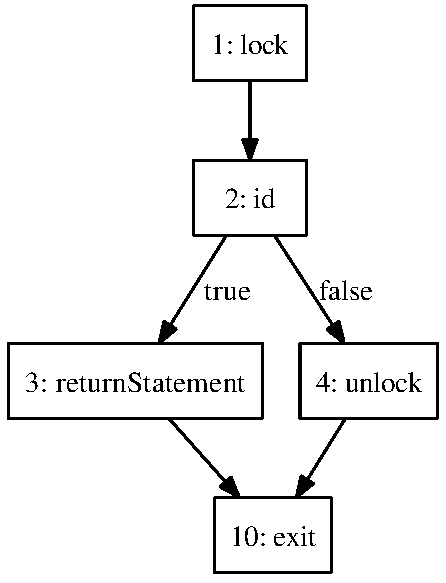
\includegraphics[width=3cm]{cfg}} & + &
  \parbox[c]{2.5cm}{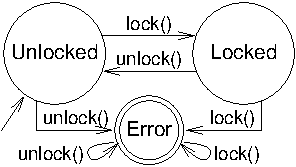
\includegraphics[width=2.5cm]{automaton}} & = &
  \parbox[c]{1.3cm}{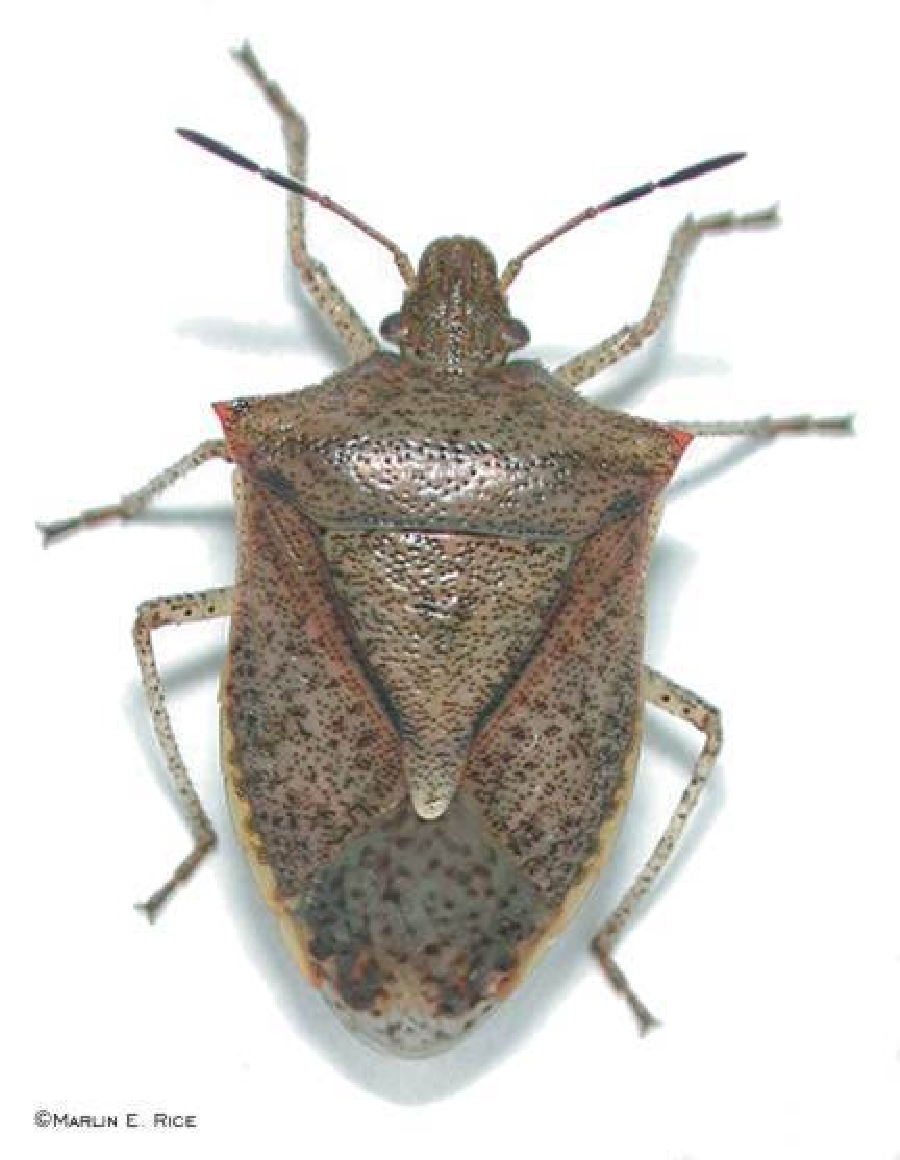
\includegraphics[width=1.3cm]{bug}} \\
  \scriptsize{Source} & & \scriptsize{CFG} & & \scriptsize{Automaton} & &
  \scriptsize{Bugs}
  \end{tabular}
  \end{center}

\end{frame}

\begin{frame}[fragile]
  \setbeamercovered{invisible}

  \frametitle{Flow Analysis Worked Example}
  \begin{center}
  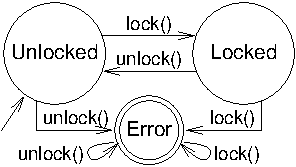
\includegraphics[width=4cm]{automaton}
  \end{center}

  \pause
  \medskip

  \scriptsize{For simplicity, instead of CFG, code is shown:}

  \bigskip

  \begin{tabular}{c|c||c|c||c|c||c}
I1 & & I2 & & I3 & & I4=I3 \\ \hline
  \begin{lstlisting}[language=C]
U
U
U
U
U
U
U
  \end{lstlisting} &
  \begin{lstlisting}[language=C]
while (X) {
  if (Y)
    lock();
  do_work();
  if (Y)
    unlock();
}
  \end{lstlisting} & \pause
  \begin{lstlisting}[language=C]
U
U
L
U,L
U,L
E,U
E,U
  \end{lstlisting} &
  \begin{lstlisting}[language=C]
while (X) {
  if (Y)
    lock();
  do_work();
  if (Y)
    unlock();
}
  \end{lstlisting} & \pause
  \begin{lstlisting}[language=C]
E,U
E,U
E,L
E,U,L
E,U,L
E,U
E,U
  \end{lstlisting} &
  \begin{lstlisting}[language=C]
while (X) {
  if (Y)
    lock();
  do_work();
  if (Y)
    unlock();
}
  \end{lstlisting} & \pause
  $\cdots$
  \end{tabular}

  \pause

  \begin{center}
  \heading{Error state (E) detected, even though the code is correct.}
  \end{center}

\end{frame}

\begin{frame}[fragile]
  \setbeamercovered{invisible}

  \frametitle{State of the Art II.}
  \begin{itemize}
  \item[(2)] Symbolic execution
  \begin{itemize}
  \item Described in 70's, but used after 2000
  \item Works on low-level code
  \item Tracks path conditions
  \begin{itemize}
    \item Uses (mostly SAT) solver
  \end{itemize}
  \item Minimum false-positives
  \item Examples: \textsc{Klee}, \textsc{Dart}
  \end{itemize}
  \end{itemize}

  \begin{center}
  \begin{tabular}{ccccccc}
  \begin{lstlisting}[language=C]
a /= b;
  \end{lstlisting} & $\Rightarrow$ &
  \begin{lstlisting}[language=XML]
%0 = sdiv %a, %b
ret %0
  \end{lstlisting} & + &
  \parbox[c]{2cm}{
    \begin{center}
    $(\varphi \wedge b = 0)$ \\
    $\vee$ \\
    $(\psi \wedge b \neq 0)$ \\
    $\Downarrow$ \\
    $b = 0?$
    \end{center}
  } & = &
  \parbox[c]{1.3cm}{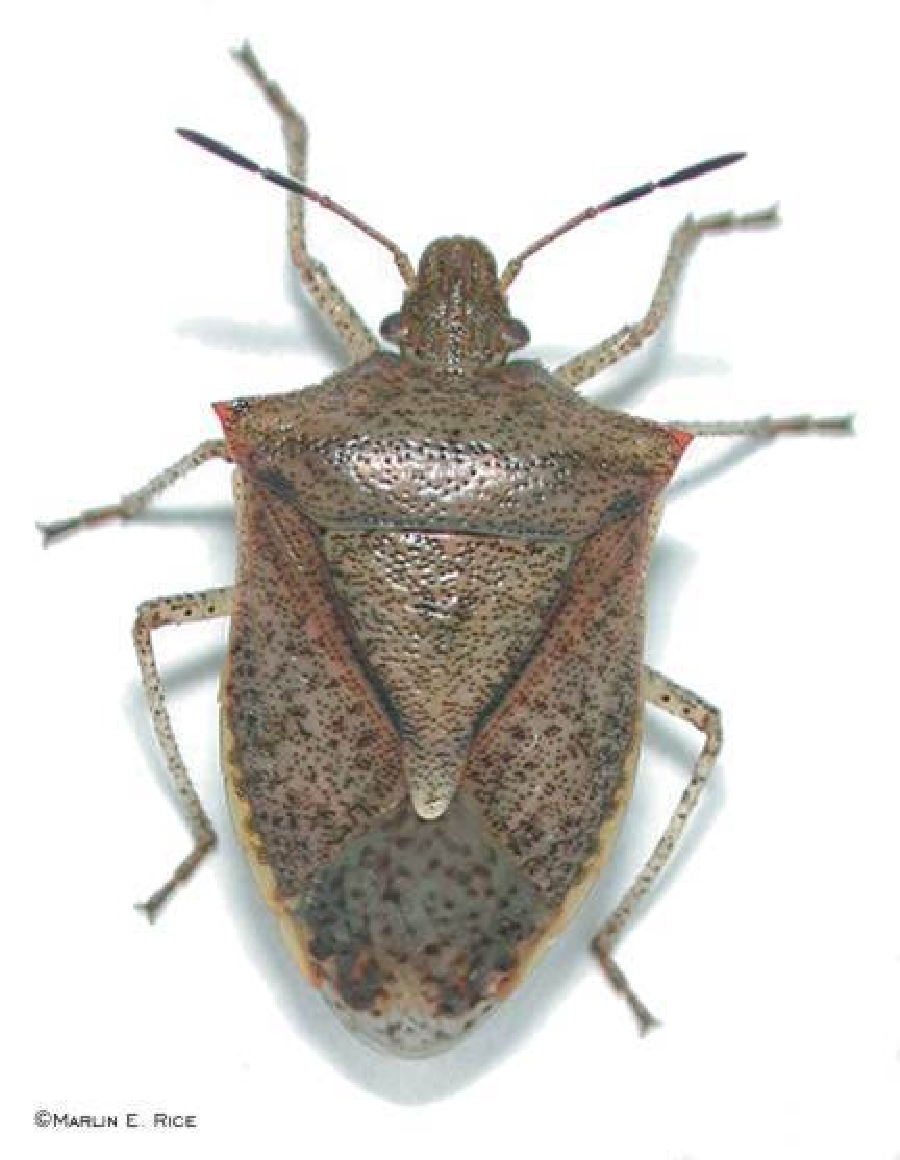
\includegraphics[width=1.3cm]{bug}} \\
  \scriptsize{Source} & & \scriptsize{Low-level code} & & \scriptsize{Solving
  path} & & \scriptsize{Bugs} \\
  & & & & \scriptsize{condition} & &
  \end{tabular}
  \end{center}

\end{frame}

\begin{frame}[fragile]
  \frametitle{Symbolic Execution Worked Example}
  \scriptsize{For simplicity, instead of low-level, normal code is shown:}

  \bigskip

  \begin{tabular}{l|l|l}
  \begin{lstlisting}[language=C]
...
while (X)
{
  if (Y)
    lock();
  do_work();
  if (Y)
    unlock();
}
...
  \end{lstlisting} &
  \parbox{3.5cm}{
\onslide<2->{$U$} \\
\onslide<2->{$U = (X \vee \neg X) \wedge U$} \\
\onslide<3->{$X \wedge U$} \\
\onslide<4->{$X \wedge U = X \wedge (Y \vee \neg Y) \wedge U$} \\
\onslide<5->{$X \wedge ((Y \wedge L) \vee (\neg Y \wedge U))$} \\
\onslide<5->{$X \wedge ((Y \wedge L) \vee (\neg Y \wedge U))$} \\
\onslide<5->{$X \wedge ((Y \wedge L) \vee (\neg Y \wedge U))$} \\
\onslide<6->{$X \wedge (Y \vee \neg Y) \wedge U = X \wedge U$} \\
\onslide<7->{$X \wedge U$} \\
\onslide<8->{$\neg X \wedge U$}
} &
  \parbox{5cm}{
\onslide<2->{initial setup, $X$ may be unknown} \\
\onslide<2->{\texttt{while} fork} \\
\onslide<3->{true branch, only $X$ remains} \\
\onslide<4->{\texttt{if} fork} \\
\onslide<5->{locked if $Y$, unlocked if not} \\
\\
\\
\onslide<6->{if $Y$, unlock} \\
\\
\onslide<8->{out of loop -- $X$ does not hold}
}
  \end{tabular}

  \medskip

  \begin{center}
  \onslide<9->{\heading{No false-positive as with Flow Analysis.}}
  \end{center}

\end{frame}

\begin{frame}
  \frametitle{State of the Art III.}
  \begin{itemize}
  \item[(3)] Model checking
  \begin{itemize}
  \item Proves math model of the code
  \item No false-positives
  \item Path explosion problem
  \item Advanced in the past decade
  \begin{itemize}
  \item Lazy abstraction
  \end{itemize}
  \item Examples: \textsc{Spin}
  \end{itemize}

  \pause

  \item[(4-)] Watching assertions, \ldots
  \begin{itemize}
  \item Very simple techniques
  \item Mostly strictly oriented
  \end{itemize}
  \end{itemize}

\end{frame}

\begin{frame}[fragile]
  \frametitle{State of the Art IV.}

  \heading{The mainstream}
  \begin{itemize}
  \item Symbolic execution
  \item Combination of techniques
  \item Lazy + abstract model checking
  \end{itemize}
  \pause
  \medskip

  \heading{Symbolic execution + Dynamic run}
  \begin{itemize}
  \item Both run concurrently
  \begin{itemize}
  \item With the same input
  \end{itemize}
  \item (Linear) solver cannot feasible compute everything
  \begin{itemize}
  \item Dynamic data used instead
  \end{itemize}
  \begin{center}
  \begin{tabular}{c}
  \begin{lstlisting}[language=C]
int compare(int x, int y) {
  return x*x == hash(y);
}
  \end{lstlisting}
  \end{tabular}
  \end{center}
  \item Examples: \textsc{Dart}, \ldots (Windows only)
  \end{itemize}

\end{frame}

\part{Kernel Checking}

\begin{frame}
  \partpage
\end{frame}

\begin{frame}[fragile]
  \frametitle{Kernel Checking I.}
  \begin{itemize}
  \item[(1)] Everyday use: \textsc{Sparse}
  \begin{itemize}
  \item Simple flow analyses
  \item Rather a parser with more checks
  \item In-kernel support (\texttt{make C=1})
  \end{itemize}
  \end{itemize}

  \begin{lstlisting}[language=C,numbers=left,numbersep=2pt]
static void bug(char __attribute__((noderef)) *x) {
  if (!x)
    *x;
}
  \end{lstlisting}
  \begin{lstlisting}[language=XML]
$ sparse source.c
source.c:3:6: warning: dereference of noderef expression
  \end{lstlisting}

  \pause

  \begin{itemize}
  \item[(2)] \textsc{Smatch}
  \begin{itemize}
  \item A more clever \textsc{Sparse}
  \item Very simple technique, unrolls loops only twice
  \item Infrastructure for code checkers
  \item Easy start (\texttt{make C=1 CHECK="smatch -p=kernel"})
  \end{itemize}
  \end{itemize}

  \begin{lstlisting}[language=XML]
$ smatch source.c
source.c +3 bug(2) error: we previously assumed 'x' could be null.
  \end{lstlisting}

\end{frame}

\begin{frame}[fragile]
  \frametitle{Kernel Checking II.}
  \begin{itemize}
  \item[(3)] \textsc{Stanse}
  \begin{itemize}
  \item Interprocedural analysis, points-to analysis
  \item Counts fix-points (unrolls loops infinitely)
  \item 4 configurable checkers
  \begin{itemize}
  \item \textsc{AutomatonChecker} -- technique above
  \item \textsc{ThreadChecker} -- combines RAGs of threads
  \item \textsc{LockChecker} -- statistics about locked variables
  \item \textsc{ReachabilityChecker} -- (un)reachable code
  \end{itemize} \pause
  \item GUI, web-frontend for errors
  \item False-positive rate is about 50\% $\Rightarrow$ not much usable
  \item Kernel supported (\texttt{make CC=stcc; stanse --jobfile jf})
  \end{itemize}
  \end{itemize} \pause

  \begin{lstlisting}[language=C,numbers=left,numbersep=2pt]
static void bug(char __attribute__((noderef)) *x) {
  if (!x)
    *x;
}
  \end{lstlisting}
  \begin{lstlisting}[language=XML]
$ stanse -c AutomatonChecker:memory.xml source.c
[0] /tmp/b.c.preproc, line 3: Dereferencing NULL pointer
error-trace [1] [locations: 2]
pointer is NULL. [file: /tmp/b.c.preproc, line: 2]
dereferencing NULL pointer here.[x] [file: /tmp/b.c.preproc, line: 3]
  \end{lstlisting}

\end{frame}

\begin{frame}
  \frametitle{Kernel Checking III.}
  \begin{itemize}
  \item[(4)] \textsc{Klee}
  \begin{itemize}
  \item Symbolic executor
  \item Accepts \textsc{LLVM} as input
  \item False-positive rate should be low
  \begin{itemize}
  \item But HW interaction!
  \end{itemize}
  \item Kernel support in (slow) progress
  \begin{itemize}
  \item LLVM compiler and linker
  \item What should be made symbolic
  \item \ldots
  \end{itemize}
  \end{itemize} \pause

  \item[(5)] \textsc{Spin}
  \begin{itemize}
  \item Model checking
  \item Much optimized
  \item One of few usable on kernel
  \item Proves locking
  \end{itemize}
  \end{itemize}

\end{frame}

\begin{frame}
  \frametitle{Kernel Checking IV.}
  \begin{itemize}
  \item[(6)] Commercial tools 
  \begin{itemize}
  \item Do much more thorough analyses
  \item Support more languages (C, C++, C\#, Java, \ldots)
  \item Are much more expensive
  \pause
  \item \textsc{Coverity}
  \begin{itemize}
  \item Scans some open-source projects (kernel included)
  \end{itemize}
  \item \textsc{Klocwork}
  \end{itemize}
  \end{itemize}

\end{frame}

\begin{frame}
  \frametitle{Checking Our Kernels}
  \heading{Pros}
  \begin{itemize}
  \item Easily get rid of some kind of bugs
  \item The infrastructure is (almost) there
  \end{itemize} \pause
  \heading{Cons}
  \begin{itemize}
  \item Who would check and walk the results?
  \item Is it worth it?
  \begin{itemize}
  \item Nobody can predict if it helps in any way
  \end{itemize}
  \end{itemize}

\end{frame}

\begin{frame}
  \frametitle{Conclusion}
  \begin{itemize}
  \item Many approaches currently used
  \begin{itemize}
  \item Flow analyses, Symbolic execution, Model checking, combination
  \end{itemize}
  \item Implemented in many various tools
  \begin{itemize}
  \item \textsc{Sparse} (FA), \textsc{Smatch} (FA), \textsc{Stanse} (FA),
  \textsc{Klee} (SE), \textsc{Spin} (MC)
  \item Their usability varies
  \item Their usability on kernel varies
  \end{itemize}
  \item Possibly, our kernels can be checked automatically
  \end{itemize}

\end{frame}

\begin{frame}
  \frametitle{Thanks}
  \begin{center} \LARGE
  Thank you for your attention! \\[2.5em]
  Questions?
  \end{center}

\end{frame}

\end{document}

